\documentclass{scrreprt}

\usepackage{aligned-overset}
\usepackage{amsmath}
\usepackage{amssymb}
\usepackage{amsthm}
\usepackage{bm}
\usepackage[shortlabels]{enumitem}
\usepackage{hyperref}
\usepackage[utf8]{inputenc}
\usepackage{multicol}
\usepackage{mathtools}
\usepackage{physics}
\usepackage{tabularx}
\usepackage{titling}
\usepackage{fancyhdr}
\usepackage{xfrac}
\usepackage{pgfplots}

\pgfplotsset{compat = newest}
\usetikzlibrary{intersections}
\usetikzlibrary{patterns}
\usetikzlibrary{positioning}
\usetikzlibrary{shapes.geometric}
\usepgfplotslibrary{fillbetween}

\newtheorem*{lemma}{Lemma}

\author{Karsten Lehmann}
\date{WiSe 2021/2022}
\title{Vorlesungsnotizen\\Lineare Algebra - Grundlegende Konzepte}

\setlength{\headheight}{26pt}
\pagestyle{fancy}
\fancyhf{}
\lhead{\thetitle}
\rhead{\theauthor}
\lfoot{\thedate}
\rfoot{Seite \thepage}

\begin{document}

\paragraph{Mengen:}
Ansammlungen verschiedener wohldefinierter Objekte, die Elemente genannte werden.

\textbf{Bsp.} Die Zahlen $1, 2, 5$ sind mathematische Objekte.
Die Menge, welche diese Objekte enthält wird geschrieben als
$\qty{1, 2, 5}$.
Dabei spielt die Reihenfolge der Elemente keine Rolle:
\[
  \qty{1, 2, 5} = \qty{2, 1, 5}
  \underset{
    \underset{
      \makebox[0pt]{\text{Mehrfachnennung möglich}}
    }\uparrow
  }= \qty{1, 2, 2, 5, 5, 5, 5, 5}
\]
Zwei Mengen heißen gleich, wenn Sie die selben Elemente haben.

\textbf{Schreibe:}
\begin{itemize}
\item $x \in M$ um auszudrücken, dass $x$ ein Element von $M$
  (in $M$ enthalten) ist.
  Zum Beispiel:
  \[
    1 \in \qty{1, 2, 5} \: 2 \in \qty{1, 2, 5}
  \]
\item $x \notin M$ um auszudrücken, dass $x$ \textbf{kein} Element von $M$ ist.
  Zum Beispiel:
  \[
    3 \notin \qty{1, 2, 5}
  \]
\end{itemize}

\subparagraph{Wichtige Mengen}
\begin{itemize}
\item $\mathbb{N}$ die Menge der natürlichen Zahlen (ohne $0$).
  \[
    \mathbb{N} = \qty{1, 2, 3, \ldots}
  \]

\item $\mathbb{N}_0$ die Menge der natürlichen Zahlen mit der $0$.
  \[
    \mathbb{N}_0 = \qty{0, 1, 2, \ldots}
  \]

\item $\mathbb{Z}$ die Menge der ganzen Zahlen.
  \[
    \mathbb{Z} = \qty{\ldots, -2, -1, 0, 1, 2, \ldots}
  \]

\item $\mathbb{Q}$ die Menge der rationalen (gebrochenen) Zahlen.
  \[
    \mathbb{Q} = \qty{\frac{p}{q} \, \middle | \, p, q \in \mathbb{Z}, q \ne 0}
  \]

\item $\mathbb{R}$ die Menge der reellen Zahlen.
\item $\mathbb{I}$ die Menge der irrationalen Zahlen.
  \[
    \mathbb{I} = \mathbb{R} \setminus \mathbb{Q}
  \]

\item $\mathbb{C}$ die Menge der komplexen Zahlen.
\end{itemize}

\textbf{Def.} Wir sagen $N$ ist eine Teilmenge von $M$ (und schreiben
$N \subseteq M$) falls jedes Element von $N$ schon Element von $M$ ist,
zum Beispiel
\[
  \qty{1, 2} \subseteq \qty{1, 2, 3} \qquad
  \mathbb{N} \subseteq \mathbb{N}_0 \subseteq \mathbb{Z}
  \subseteq \mathbb{Q} \subseteq \mathbb{R} \subseteq \mathbb{C}
\]

\textbf{Beachte:} Sind $M, N$ Mengen, dann gilt
\[
  M = N \iff M \subseteq N \land N \subseteq M
\]
(wird oft genutzt um zu zeigen, dass zwei Mengen gleich sind)

\subparagraph{Teilmengen} können durch eine auszeichnende Eigenschaft beschrieben werden.
Zum Beispiel
\begin{itemize}
\item $\qty\Big{z \in \mathbb{Z} \, {\Big |} \, 2 \text{ teilt } z}$
  ist die Menge der geraden ganzen Zahlen.

\item $\qty\Big{i \in \mathbb{Z} \, {\Big |} \, i \geq -5}$
  ist die Menge der ganzen Zahlen, welche größer oder gleich $5$ sind.

\item $\qty\Big{i \in \mathbb{N} \, {\Big |} \, i \leq 8} =
  \qty{1, 2, 3, 4, 5, 6, 7, 8}$
\end{itemize}

Manchmal schreibt man abkürzend
\begin{itemize}
\item $\mathbb{N} = \qty{1, 2, 3, \ldots}$
\item $\qty\Big{i \in \mathbb{Z} \, {\Big |} \, i \geq -5} = \qty{-5, -4, -3, \ldots}$
\item $\qty\Big{i \in \mathbb{Z} \, {\Big |} \, i \leq 8} = \qty{1, \ldots, 8}$
\end{itemize}

Andere mögliche Schreibweisen sind
\begin{itemize}
\item $\qty\Big{z \in \mathbb{Z} \, {\Big |} \, 2 \text{ teilt } z} =
  \qty\Big{2x \, {\Big |} \, x \in \mathbb{Z}}$

\item $\mathbb{Q} =
  \qty{\frac{p}{q} \, \middle | \, p, q \in \mathbb{Z}, q \ne 0}$
\end{itemize}

Es gibt genau eine Menge welche gar keine Elemente enthält, nämlich die leere
Menge - geschrieben als $\qty{}$ oder $\emptyset$.
\\

Mengen selbst sind wieder mathematische Objekte und können damit Elemente
einer Menge sein, zum Beispiel
\begin{itemize}
\item $\qty{\emptyset, \mathbb{N}}$ ist die Menge, welche die leere Menge und
  die Menge der natürlichen Zahlen enthält.

\item die Menge $\qty\Big{\qty{1, 2, 5}}$ hat nur ein Element, nämlich die Menge
  $\qty{1, 2, 5}$.
\end{itemize}

Für jede Menge $M$ gilt $\emptyset \subseteq M$.
In vielen Fällen gilt allerdings $\emptyset \notin M$,
so zum Beispiel $\emptyset \notin \qty{1, 2, 5}$.
\begin{itemize}
\item $\qty\Big{1, 2, \qty{5, 6}} \ne \qty{1, 2, 5, 6}$
\end{itemize}

Ist $M$ eine Menge, so schreibt man $P(M)$ (manchmal auch $2^M$)
für die Menge deren Elemente alle Teilmengen von $M$ sind.
Man nennt $P(M)$ die \textbf{Potenzmenge} von $M$.
Es gilt immer $\emptyset \subseteq P(M)$.

\textbf{Bsp.:}
\begin{itemize}
\item $P(\qty{1, 2}) = \qty\Big{\emptyset, \qty{1}, \qty{2}, \qty{1, 2}}$
\item $P(\qty{1, 2, 3}) =
  \qty\Big{\emptyset, \qty{1}, \qty{2}, \qty{3}, \qty{1, 2}, \qty{1, 3},
    \qty{2, 3}, \qty{1, 2, 3}}$
\end{itemize}

Hat die Menge $M$ insgesamt $n$ Elemente, so ist $\abs{P(M)} = 2^n$.
Außerdem ist $P(\emptyset) = \qty{\emptyset}$.

\subparagraph{Mengenoperatoren}
Sind $M$ und $N$ Mengen, so schreibt man
\begin{itemize}
\item $M \cap N$ für den \emph{Durchschnitt} der Mengen $M$ und $N$,
  dass heißt für die Menge aller Objekte, die sowohl ein Element von
  $M$ als auch von $N$ sind.
  \[
    M \cap N = \qty\Big{x \, {\Big |} \, x \in M \land x \in N}
  \]
  \begin{tikzpicture}
    \node at (-0.5, 2) (label_m) {$M$};
    \node at (4, 2) (label_n) {$N$};
    \node at (2, -2) (label_mn) {$M \cap N$};
    \node[circle, draw, minimum size=3cm] at (1, 0) (set_m) {};
    \node[circle, draw, minimum size=3cm] at (3, 0) (set_n) {};
    \draw[->] (label_m) -- (set_m.center);
    \draw[->] (label_n) -- (set_n.center);
    \begin{scope}
      \clip (1, 0) circle (1.5cm);
      \fill[pattern color=red, pattern=north west lines] (3, 0) circle (1.5cm);
    \end{scope}
    \draw[->] (label_mn) -- (2, 0);
  \end{tikzpicture}

\item $M \cup N$ für die Vereinigung von $M$ und $N$.
  Das ist die Menge aller mathematischen Objekte, die ein Element von $M$
  oder $N$ sind.

  \begin{tikzpicture}
    \node at (-0.5, 2) (label_m) {$M$};
    \node at (4, 2) (label_n) {$N$};
    \node at (2, -2) (label_mn) {$M \cup N$};
    \node[circle, draw, minimum size=3cm, pattern color=red, pattern=north west lines] at (1, 0) (set_m) {};
    \node[circle, draw, minimum size=3cm, pattern color=red, pattern=north west lines] at (3, 0) (set_n) {};
    \draw[->] (label_m) -- (set_m.center);
    \draw[->] (label_n) -- (set_n.center);
    \draw[->] (label_mn) -- (2, 0);
  \end{tikzpicture}

\item $M \setminus N$ für das Komplement von $N$ in $M$.

  \begin{tikzpicture}
    \node at (-0.5, 2) (label_m) {$M$};
    \node at (4, 2) (label_n) {$N$};
    \node at (2, -2) (label_mn) {$M \setminus N$};
    \node[circle, draw, minimum size=3cm] at (1, 0) (set_m) {};
    \node[circle, draw, minimum size=3cm] at (3, 0) (set_n) {};
    \draw[->] (label_m) -- (set_m.center);
    \draw[->] (label_n) -- (set_n.center);
    \begin{scope}
      \clip (1, 0) circle (1.5cm);
      \fill[even odd rule, pattern color=red, pattern=north west lines] (3, 0) circle (1.5cm) (1, 0) circle (1.5cm);
    \end{scope}
    \draw[->] (label_mn) -- (1.25, -1);
  \end{tikzpicture}
\end{itemize}

\newpage
Beispiele
\begin{itemize}
\item $\qty{1, 2, 3} \cap \qty{1, 2, 5} = \qty{1, 2}$
\item $\qty{1, 2, 3} \cup \qty{1, 2, 5} = \qty{1, 2, 3, 5}$
\item $\mathbb{N}_0 \cup \qty{-1, -2, -3, \ldots} = \mathbb{Z}$
\item $\qty\Big{z \in \mathbb{Z} \, {\Big |}
    \, 2 \text{ teilt } z} \cap \mathbb{N}_0 =
  \qty\Big{n \in \mathbb{N}_0 \, {\Big |} \, 2 \text{ teilt } n}$
\item $\qty\Big{z \in \mathbb{Z} \, {\Big |}
    \, 2 \text{ teilt } z} \cup \mathbb{N}_0 =
  \qty{\ldots, -4, -2, 0, 1, 2, 3, \ldots}$
\item $\qty{1, 2, 3} \setminus \qty{1, 2} = \qty{3}$
\end{itemize}

Sei $I$ eine Indexmenge (dass heißt für jedes $i \in I$ sei $M_i$ eine Menge).
Dann heißt
\begin{enumerate}[$\Rightarrow$]
\item $\underset{i \in I}\bigcap M_i \underset{
    \underset{
      \makebox[0pt]{ist definiert als}
    }{\Big\uparrow}
  }\coloneqq \qty\Big{x \, {\Big |} \, x \in M_i \forall i \in I}$
  der Durchschnitt der $M_i, i \in I$.

\item $\underset{i \in I}\bigcap M_i \coloneqq
  \qty\Big{x \, {\Big |} \, x \in M_i \forall i \in I}$
  die Vereinigungsmenge der $M_i, i \in I$.
\end{enumerate}

\textbf{Beispiel:}
\begin{itemize}
\item $I = \mathbb{N}, M_i =
  \qty\Big{n \in \mathbb{N} \, {\Big |} \, n \leq i}$
  \begin{flalign*}
    &\bigcap_{i \in I} M_i = \qty{1} \quad \bigcup_{i \in I} M_i = \mathbb{N}&
  \end{flalign*}

\item $I = \qty{1, 2, 3, \ldots, n}, n \in \mathbb{N}, M_i =
  \qty\Big{n \in \mathbb{N} \, {\Big |} \, n \leq i}$
  \begin{flalign*}
    \bigcap_{i \in I} M_i &= M_1 \cap M_2 \cap \ldots \cap M_n = \qty{1} & \\
    \bigcup_{i \in I} M_i &= M_1 \cup M_2 \cup \ldots \cup M_n = I
  \end{flalign*}
\end{itemize}

Eine Menge heißt \emph{endlich}, falls $n \in \mathbb{N}_0$ existiert und
$x_1, \ldots, x_n$ mit $M = \qty{x_1, \ldots, x_n}$.

Wenn $x_i \ne x_j$ ist für $i \ne j$, dann ist $n$ die Anzahl der Elemente von
$M$, auch \emph{Kardinalität} genannt, geschrieben als $\abs{M}$, zum Beispiel:

\[
  \abs\big{\qty{1, 2, \ldots, n}} = n \qquad
  \abs\Big{\qty\big{\emptyset, \qty{1, 2}}} = 2 \qquad
  \abs\big{\qty{1, 2, 2}} = 2
\]

$\mathbb{N}, \mathbb{N}_0, \mathbb{Z}, \mathbb{Q}, \mathbb{R}, \mathbb{C}$ sind
nicht endlich, das heißt \emph{unendlich}.

\newpage
\paragraph{Tupel}
Wenn $M = \qty{x_1, \ldots, x_n}$ eine Menge ist, macht die Reihenfolge
beziehungsweise Wiederholung von Elementen keinen Unterschied.
Falls Reihenfolge/Wiederholung von Elementen einen Unterschied machen sollen,
dann schreibt man ein \emph{Tupel} $\qty\big(x_1, x_2, \ldots, x_n)$.

Zwei Tupel $\qty\big(x_1, \ldots, x_n)$ und $\qty\big(y_1, \ldots, y_n)$ heißen
gleich, falls $x_i = y_i$ für alle $i \in \qty{1, \ldots, n}$ gilt, zum Beispiel
\begin{flalign*}
  \qty(1, 2, 2) \ne \qty(1, 2) &\text{ aber } \qty{1, 2, 2} = \qty{1, 2} & \\
  \qty(1, 2, 3) \ne \qty(3, 2, 1) &\text{ aber} \qty{1, 2, 3} = \qty{3, 2, 1}
\end{flalign*}
Ein Tupel mit zwei Einträgen (das heißt der Form $\qty\big(x_1, x_2)$) heißt Paar.
Ein Tupel $\qty\big(x_1, \ldots, x_n)$ heißt $n$-Tupel.

Wenn Mengen $M_1, \ldots, M_n$ gegeben sind, dann schreibt man
\[
  M_1 \times M_2 \times \ldots \times M_n =
  \qty\Big{
    \qty\big(x_1, \ldots, x_n) {\Big |}
    x_i \in M_i \, \forall \, i \in \qty\big{1, \ldots, n}
  }
\]
Zum Beispiel
$M_1 \times M_2 = \qty\Big{
\qty\big(x_1, x_2) {\Big |} x_1 \in M_1 \text{ und } x_2 \in M_2)}$.

Manchmal betrachtet man auch \emph{unendliche Tupel}
$\qty\big(x_1, x_2, x_3, \ldots)$ mit einem Eintrag $x_i$ für jedes
$i \in \mathbb{N}_0$.
Zwei unendliche Tupel $\qty\big(x_1, x_2, x_3, \ldots)$ und
$\qty\big(y_1, y_2, y_3, \ldots)$ sind gleich, falls
$x_i = y_i$ für alle $i \in \mathbb{N}_0$.

Die Schreibweise $i = 1, \ldots, n$ bedeutet $i \in \qty{1, \ldots, n}$.

\paragraph{Russellsche Antinomie} Versuche eine Menge $M$ zu definieren als
$M = \qty\big{x {\big |} x \notin x}$.

\textbf{Frage:} Gilt $M \in M$?

\textbf{Falls ja}: dann $M \notin M$ nach der Definition von $M$.
Ein Widerspruch.

\textbf{Falls nein}: dann $M \in M$ nach der Definition von $M$.
Ein Widerspruch.

\textbf{Fazit}: Es ist problematisch die Menge $M$ wie vorher zu definieren.

Um Probleme dieser Art zu vermeiden wurde die \emph{axiomatische Mengenlehre}
entwickelt.
Probleme dieser Art treten nicht auf, wenn man Teilmengen bekannter Mengen
bildet, zum Beispiel ist $M = \qty\big{x \in \mathbb{N} {\big |} x \notin x}$
wohldefiniert und $M = \mathbb{N}$

\section*{Aussagenlogik}

Aussagen sind zum Beispiel ``\emph{Der Himmel ist blau}'' oder
``\emph{Katzen sind schwarz}'' oder ``$1 + 2 = 3$'' oder
``$4 = 5$''.
Aussagen können entweder \emph{wahr} oder \emph{falsch} sein.

Wenn zwei Aussagen $A$ und $B$ gegeben sind, kann man daraus weitere Aussagen
bilden:
\begin{itemize}
\item ``$A$ oder $B$'' (geschrieben $A \lor B$)
\item ``$A$ und $B$'' (geschrieben $A \land B$)
\item ``nicht $A$'' (geschrieben $\neg A$)
\end{itemize}

Bei dem ``oder'' handelt es sich um das ``nicht-ausschließliche''
(inklusive) oder, dass heißt $A$ oder $B$ ist auch wahr, falls
$A$ und $B$ beide wahr sind.

\newpage
Schreibe F für ``falsch'' und W für ``wahr''.
\begin{center}
  \begin{tabular}{c | c | c | c | c}
    $A$ & $B$ & $A \lor B$ & $A \land B$ & $\neg A$ \\
    \hline
    W & W & W & W & F \\
    W & F & W & F & F \\
    F & W & W & F & W \\
    F & F & F & F & F
  \end{tabular}
\end{center}

$\qty(\neg A) \lor B$ kürzt man ab als $A \Rightarrow B$ und man sagt dafür
``$A$ impliziert $B$'' oder ``aus $A$ folgt $B$''.

Man schreib $A \iff B$ für die Aussage
$\qty(A \Rightarrow B) \iff \qty(B \Rightarrow A)$ und sagt ``$A$ und $B$ sind
äquivalent'' oder ``$A$ gilt genau dann, wenn $B$ gilt'' - kurz ``$A$ gdw. $B$''.

\begin{center}
  \begin{tabular}{c | c | c | c}
    $A$ & $B$ & $A \Rightarrow B$ & $A \iff B$ \\
    \hline
    W & W & W & W \\
    W & F & F & F \\
    F & W & W & F \\
    F & F & F & F
  \end{tabular}
\end{center}

\textbf{Wichtig:} Ist $A$ falsch, so ist die Aussage $A \Rightarrow B$ immer
wahr! ``ex falso quodlibet'' (lat. aus Falschem folgt Beliebiges), zum Beispiel
ist die Aussage $2 = 3 \Rightarrow 5 = 100$ wahr.
Genauso ist $A \iff B$ auch dann wahr, wenn $A$ und $B$ falsch sind.

\subparagraph{Tautologie} Eine Tautologie ist eine ``zusammengesetzte Aussage'',
die unabhängig von ihren Teilaussagen immer wahr ist, zum Beispiel sind
$\qty(\neg A) \lor A$ oder $A \land B \Rightarrow A$ oder $A \iff A$
Tautologien.

\textbf{Wichtige Tautologien:}
\begin{enumerate}[(1)]
\item $\neg(\neg A) \iff A$
\item $(A \lor B) \iff (B \lor A)$
\item $(A \land B) \iff (B \land A)$
\item
  \label{taut_4}
  $\qty\big((A \Rightarrow B) \land (B \Rightarrow C))
  \Rightarrow (A \Rightarrow C)$
\end{enumerate}

In der Praxis kann man $A \Rightarrow B$ oft zeigen, indem man Aussagen
$A_1 = A, A_2, \ldots, A_n = B$ findet, so dass $A_i \Rightarrow A_{i + 1}$
für alle $i = 1, \ldots, n - 1$ wahr ist.
In dem man $\hyperref[taut_4]{(4)}$ wiederholt anwendet, weiß man dann, dass
$A \Rightarrow B$ wahr ist.
Man nennt dieses Verfahren einen \emph{Kettenschluss}.

Man sagt, dass Aussagen $A_1, \ldots, A_n$ äquivalent sind, falls
$A_i \iff Aj$ für alle $i, j \in \qty{1, \ldots, n}$.
Äquivalent dazu ist, dass die Implikation $A_i \Rightarrow A_{i + 1}$ für
alle $i = 1, \ldots, n - 1$ und $A_n \Rightarrow A_1$ wahr sind.

\paragraph{Äquivalenzrelation} Sei $\sim$ eine Äquivalenzrelation auf einer
Menge $M$, dass heißt
\begin{itemize}
\item $\sim$ ist eine Relation auf $M$
\item $\forall x \in M \colon x \sim x$ (Reflexivität)
\item $\forall x, y \in M \colon x \sim y \Rightarrow y \sim x$
\item $\forall x, y, z \in M \colon x \sim y \land y \sim z \Rightarrow x \sim z$
\end{itemize}

Für $x \in M$ setze
\[
  \qty[x] \coloneqq \qty\Big{ y \in M {\Big |} x \sim y} \subset M
\]
und nenne $\qty[x]$ die \emph{Äquivalenzklasse} von $x$
(in $M$ bezüglich $\sim$).

Setze
\[
  M_{/ \sim} \coloneqq \qty\Big{\qty[x] {\Big |} x \in M}
  \subset \mathcal{P}(M)
\]

\textbf{Beachte:} Es kann $x, y \in M$ existieren mit $x \ne y$ und
$\qty[x] = \qty[y]$.

\begin{lemma}
  Sei $\sim$ eine Äquivalenzrelation auf $M$.
  Dann:
  \begin{enumerate}[(a)]
  \item $x \in \qty[x]$
  \item $\qty[x] = \qty[y] \iff x \sim y$
  \item $a \sim b$ für alle $a, b \in [x]$
  \item $M = \underset{x \in M}\bigcup [x]$
  \item $\qty[x] = \qty[y]$ oder $\qty[x] \cap \qty[y] = \emptyset$
  \end{enumerate}
\end{lemma}

\underline{Beweis:} Siehe das Hausaufgabenblatt 03 Analysis.

\textbf{Def.} Sei $M$ eine Menge und $P \in \mathcal{P}(M)$.
Setze $\bigcup P \coloneqq \qty\Big{ x \in M {\Big |}
  \exists N \in P \colon x \in N}$.
Die Menge $P$ wird eine Partition genannt, falls
\begin{itemize}
\item $\bigcup P = M$
\item $\forall N_1, N_2 \in P \colon N_1 = N_2 \lor N_1 \cap N_2 = \emptyset$
\item $\emptyset \notin P$
\end{itemize}

\underline{Beispiel:} $M = \qty{1, 2, 3, 4}$.
Dann sind zum Beispiel die folgenden Mengen Partitionen von $M$:
\begin{multicols}{2}
  \begin{itemize}
  \item $\qty\big{\qty{1, 2}, \qty{3, 4}}$
  \item $\qty\big{\qty{1, 3, 4}, \qty{2}}$
  \item $\qty\big{\qty{1, 2}, \qty{3}, \qty{4}}$
  \item $\qty\big{\qty{1, 2, 3, 4}}$
  \end{itemize}
\end{multicols}

Ist $M$ eine nichtleere Menge, so sind immer $\qty{M}$ und
$\qty\big{\qty[x] {\big |} x \in M}$ Partitionen.

Ist $\sim$ eine Äquivalenzrelation auf $M$, so ist $M_{/\sim}$
immer eine Partition.

Die leere Menge ist die einzige Partition der leeren Menge.

\begin{lemma}
  Sei $P$ eine Partition auf $M$ und
  \[
    R = \qty\Big{ \qty(x, y) {\Big |} \exists N \in P \colon x, y \in N}
  \]
  Dann ist $R$ eine Äquivalenzrelation auf $M$ und $M_{/R} = P$.
\end{lemma}

\underline{Beweis:} Siehe das Hausaufgabenblatt 03 Analysis.

\paragraph{Abbildungen}:
Seien $M, N$ Mengen.
Eine Abbildung (oder Funktion) von $M$ nach $N$ ist eine Zuordnung
$f \colon M \to N$, die jedem Element $m \in M$ genau ein Element
$n \in N$ zuordnet.
Manchmal schreibt man $m \mapsto n$ um auszudrücken, dass $n = f(m)$ gilt.
Formal wird eine Abbildung $f \colon M \to N$ als eine Relation
$f \subseteq M \times M$ definiert, so dass für jedes Element $m \in M$
genau ein $n \in N$ existiert mit $\qty(m, n) \in f$.
Dann ist $f(m)$ das eindeutige Element von $N$ mit $\qty(m, f(m)) \in f$.

Von nun an sei $f \colon M \to N$ immer eine Abbildung.
Für $T \subseteq M$ setze $f(T) = \qty\Big{f(t) {\Big |} t \in T}$.

\begin{center}
  \begin{tikzpicture}
    \node[
      draw,
      ellipse,
      minimum height = 3.5cm,
      minimum width = 1.75cm,
      ] at (0, 0) (M) {};
    \node[
      draw,
      ellipse,
      minimum height = 3.5cm,
      minimum width = 1.75cm,
    ] at (4, 0) (N) {};
    \node[
      circle,
      fill,
      inner sep=1pt,
      label=$m_1$,
    ] at (-0.25, 0.5) (m1) {};
    \node[
      circle,
      fill,
      inner sep=1pt,
      label=left:$m_2$,
    ] at (0.3, 0.2) (m2) {};
    \node[
      circle,
      fill,
      inner sep=1pt,
      label=$m_3$,
    ] at (-0.25, -0.6) (m3) {};
    \node[
      circle,
      fill,
      inner sep=1pt,
      label=$m_4$,
    ] at (0.3, -1.2) (m4) {};
    \node[
      circle,
      fill,
      inner sep=1pt,
      label=$n_1$,
    ] at (3.75, 0.5) (n1) {};
    \node[
      circle,
      fill,
      inner sep=1pt,
      label=$n_2$,
    ] at (4.3, 0.2) (n2) {};
    \node[
      circle,
      fill,
      inner sep=1pt,
      label=$n_3$,
    ] at (4, -0.7) (n3) {};
    \node[
      circle,
      draw,
      inner sep=4.5mm
    ] at (0, 0.55) (T) {};
    \node[
      circle,
      draw,
      inner sep=4.5mm
    ] at (4, 0.55) (fT) {};
    \node[
      below left = 0cm of M,
    ] {$M$};
    \node[
      below right = 0cm of N,
    ] {$N$};
    \node[
      above left = -0.2cm  and 0.2 of T,
    ] {$T$};
    \node[
      above right = -0.2cm  and 0.2 of fT,
    ] {$f(T)$};
    \draw[->] (m1) -- (n2);
    \draw[->] (m2) -- (n1);
    \draw[->] (m3) -- (n3);
    \draw[->] (m4) -- (n3);
  \end{tikzpicture}
\end{center}

Bild von $f = \text{Bild}(f) = f(M)$.

Bild von $T$ unter $f = f(T)$.

Für $x \in M$ nenne $f(x)$ das Bild von $x$ unter $f$ und $x$ ein Urbild von
$f(x)$ unter $f$.

Ist $S \subseteq N$, so nenne
$f^{-1}(S) \coloneqq \qty\Big{x \in M {\Big |} f(x) \in S}$ das Urbild von $S$
unter $f$.

\begin{center}
  \begin{tikzpicture}
    \node[
      draw,
      ellipse,
      minimum height = 3.5cm,
      minimum width = 1.75cm,
      ] at (0, 0) (M) {};
    \node[
      draw,
      ellipse,
      minimum height = 3.5cm,
      minimum width = 1.75cm,
    ] at (4, 0) (N) {};
    \node[
      circle,
      fill,
      inner sep=1pt,
      label=$m_1$,
    ] at (-0.25, 0.5) (m1) {};
    \node[
      circle,
      fill,
      inner sep=1pt,
      label=left:$m_2$,
    ] at (0.3, 0.2) (m2) {};
    \node[
      circle,
      fill,
      inner sep=1pt,
      label=below:$m_3$,
    ] at (0.25, 1) (m3) {};
    \node[
      circle,
      fill,
      inner sep=1pt,
      label=$m_4$,
    ] at (-0.25, -0.6) (m4) {};
    \node[
      circle,
      fill,
      inner sep=1pt,
      label=$m_5$,
    ] at (0.3, -1.2) (m5) {};
    \node[
      circle,
      fill,
      inner sep=1pt,
      label=$n_1$,
    ] at (3.75, 0.5) (n1) {};
    \node[
      circle,
      fill,
      inner sep=1pt,
      label=$n_2$,
    ] at (4.3, 0.2) (n2) {};
    \node[
      circle,
      fill,
      inner sep=1pt,
      label=$n_3$,
    ] at (4, -0.7) (n3) {};
    \node[
      circle,
      draw,
      inner sep=4.5mm
    ] at (0, 0.55) (fS) {};
    \node[
      circle,
      draw,
      inner sep=4.5mm
    ] at (4, 0.55) (S) {};
    \node[
      below left = 0cm of M,
    ] {$M$};
    \node[
      below right = 0cm of N,
    ] {$N$};
    \node[
      above left = -0.2cm  and 0.2 of fS,
    ] {$f^{-1}(S)$};
    \node[
      above right = -0.2cm  and 0.2 of S,
    ] {$S$};
    \draw[->] (m1) -- (n1);
    \draw[->] (m2) -- (n2);
    \draw[->] (m3) -- (n1);
    \draw[->] (m4) -- (n3);
    \draw[->] (m5) -- (n3);
  \end{tikzpicture}
\end{center}

Sind $f \colon M \to N$ und $g \colon N \to L$ Abbildungen, so ist $g \circ f$
die Abbildung $g \circ f \colon M \to L$ mit $(g \circ f)(x) = g\qty\big(f(x))$
für alle $x \in M$.

Ist $f'$ eine weitere Abbildung, so heißen $f$ und $f'$ gleich, falls
$f(x) = f'(x) \; \forall \; x \in M$.

\newpage
\textbf{Def,:} Eine Abbildung $f \colon M \to N$ heißt
\begin{itemize}
\item[\underline{surjektiv:}] falls $\text{Bild}(f) = N$, dass heißt für
  jedes $n \in N$ existiert ein $m \in M$ mit $f(m) = n$.

\item[\underline{injektiv:}] falls jedes Element von $N$ höchstens ein Urbild
  hat, dass heißt \\
  $\forall x, y \in M \colon f(x) = f(y) \iff x = y$.

\item[\underline{bijektiv:}] falls die Abbildung injektiv und surjektiv ist.
\end{itemize}

Für $T \subseteq M$ und $f \colon M \to N$ definiert
$\overset{\makebox[0pt]{$f$ eingeschränkt auf $T$}}{\overbrace{f_{|T}}}$
durch $f_{|T} \colon T \to N$ mit $f_{|T}(t) = f(t)$ für alle $t \in T$ die
Einschränkung von $f$ auf $T$.

\begin{lemma}
  Seien $M, N, L$ Mengen und $f \colon M \to N, g \colon N \to L$ Abbildungen.
  Dann gilt
  \begin{enumerate}[(a)]
  \item Sind $f$ und $g$ injektiv, so ist $g \circ f$ injektiv
  \item Sind $f$ und $g$ surjektiv, so ist $g \circ f$ surjektiv
  \item Sind $f$ und $g$ bijektiv, so ist $g \circ f$ bijektiv
  \end{enumerate}
\end{lemma}

\underline{Beweis:}
\begin{enumerate}[(a)]
\item Seien $f, g$ injektiv: Sei $x, y \in M$ mit
  $(g \circ f)(x) = (g \circ f)(y)$.

  Zu zeigen: $x = y$

  Es gilt $g(f(x)) = g(f(y))$.
  Weil $g$ injektiv ist, folgt $f(x) = f(y)$.
  Weil $f$ injektiv ist, folgt $x = y$.

\item Seien $f, g$ surjektiv und $l \in L$.
  Weil $g$ surjektiv ist, existiert $n \in N$ mit
  $g(n) = l$.
  Weil $f$ surjektiv ist, existiert $m \in M$ mit
  $f(m) = n$.

  $\Rightarrow g(f(m)) = l$

  $\Rightarrow (g \circ f)(m) = l$

\item folgt aus (a) und (b)
\end{enumerate}

\end{document}